\documentclass[conference]{IEEEtran}
\IEEEoverridecommandlockouts
% The preceding line is only needed to identify funding in the first footnote. If that is unneeded, please comment it out.
% \usepackage{cite}
\usepackage{amsmath,amssymb,amsfonts}
\usepackage{comment}
\usepackage{algorithmic}
\usepackage{graphicx}
\usepackage{textcomp}
\usepackage{xcolor}
\def\BibTeX{{\rm B\kern-.05em{\sc i\kern-.025em b}\kern-.08em
    T\kern-.1667em\lower.7ex\hbox{E}\kern-.125emX}}
\usepackage[
backend=biber,
style=ieee,
sorting=ynt
]{biblatex}
\addbibresource{export.bib}
\begin{document}

\title{Literature Review for ML/DL and how it relates to Embedded Systems\\}

\author{
\IEEEauthorblockN{Seán Ó Fithcheallaigh (B00830189)}
\IEEEauthorblockA{\textit{Department of Computing} \\
\textit{Ulster University}\\
Belfast, N. Ireland \\
o\_fithcheallaigh-s@ulster.ac.uk}
}

\maketitle

\begin{abstract}
This document will be a literature review on the topic of Machine Learning and Deep Learning, and how they relate to the world of embedded systems, edge computing and ML/DL operating on constrained devices. 

This work relates to my MSc Research project, but it is mainly for my own use, and as such will not be included in the main research article submission, but may be added into the supporting material.
\end{abstract}

\begin{IEEEkeywords}
Machine Learning, Deep Learning, Embedded Systems, The Edge
\end{IEEEkeywords}

\section{Introduction}
The world is becoming a more and more connected place, with over 75 billion connected devices predicted by 2025 \cite{statista1}. Connected devices are an ecosystem of hardware and software elements which are used to connect to the physical world through the use of onboard sensors as well as connecting to the Internet. Typically, connected devices will have constrained computing power, a smaller amount of memory than would be typical on larger computing systems. Another common aspect of connected devices is they tend to be battery powered. The "Internet of Things (IoT)" is often used as a umbrella term to describe a wide range of sensor enabled devices which are also connected to the Internet.

Due to the restricted memory associated with many of these connected devices, coupled with the potential power issues, there is a need to understand how artificial intelligence (AI)\footnote{Here, AI, or artificial intelligence is used to cover the worlds of ML and DL} models can be designed to operate at the edge.

Terms like "the edge", or "edge computing" are somewhat vague, and here is a good point to try and wrap some sort of definition around them, and understand where they come from. 

As has been discussed, with the increasing development of the IoT, more and more devices are being connected to the Internet, which has resulted in large amounts of data being generated. This has resulted in problems for cloud computing services, which now struggle to to support the needs of a more connected society, in terms of things like data processing and data storage. And it is into this gap that edge technologies have emerged. The high-level, one liner to describe edge computing is a new model of computing for preforming calculations at the edge of the network. In other words, the calculations are done closer to the system user, and closet to the source of the data which is being processed \cite{Cao2020}. This new model, of course, brings it own challenges, some of which have been introduced above. 

This paper is intended to serve a number of functions. First, it will be a review of the main AI models which are common or popular today, with a focus on models used for classification tasks, since object or obstacle detection is a classification task. Second, it will be a review of literature as it relates to object detection, and to machine learning at the edge.

A number of other topics will be discussed throughout this work as they are closely related to the topics of constrained devices. Some of these have already been introduced, such as the Internet of Things, and edge computing. While these topics will be discussed throughout, not a lot of time will be given over to exploring their origins, or going into a lot of details on the research being carried out in the respective areas. 

\section{Artificial Intelligence, Machine Learning, and Deep Leaning}
In this section, we will aim to review the worlds of Artificial Intelligence (AI), machine Learning (ML) and Deep Learning (DL), and try to understand the similarities, and the differences when looking at ML and DL.

\begin{comment}
\subsection{Machine Learning Algorithms}
There are three types of ML: \textbf{Supervised Learning}, \textbf{Unsupervised Learning} and \textbf{Reinforcement Learning}. The goal of supervised learning is to learn a model with data that has already been labelled, and then pass unseen data through the model to allow it to make predictions \cite{pythonML}. The term supervised is used to refer to training data where the desired outputs are already known in advance. We can think of this like a parent teaching their child how to tell the difference between cats and dogs. The parents knows how to tell the difference between cats and dogs, and can therefore teach, or to use the correct ML terminology, train the child to tell the differences too. 

When working in in unsupervised learning, we are dealing with data that is unlabelled, and data that has an unknown structure. The techniques used in unsupervised learning allow an exploration of the data, which should lead to the extraction of important data \cite{pythonML}. A common technique used in unsupervised learning is clustering. Clustering is a method used to group elements of data into meaningful sets or collections. As an example, we can think of someone sorting their non fiction books. They might create a collection of their political groups, another collection of their biographies. They may also have another collection for their history books, and so on. The same thing is done when using clustering techniques on unsupervised data \cite{google1}.  

We will not discuss reinforcement learning here. 
\end{comment}

% \subsubsection{Artificial Intelligence, Machine Learning, and Deep Leaning}
Many people probably think they know what artificial intelligence is. As humans, we know, generally speaking, what intelligence is (we hope we have some of it), and artificial intelligence is a computerised version of human intelligence. But sometimes it is good to try and put a more formal definition around a topic, and this topic is no different. 

John McCarthy was a a computer science professor at Stanford university, he was interested in human level intelligence since the late 1940s, and in 1955, he coined the term "artificial intelligence". Throughout his career, Prof. McCarthy made a number of contributions to the field of AI, and received numerous awards related to AI \cite{mccarthy1}. 

In his paper 2007 paper \textit{What Is Artificial Intelligence} \cite{whatisai_mccarthy} Prof. McCarthy offers a definition we can use here. He says artificial intelligence is the process of using science and engineering to make intelligent machines, with a focus on intelligent computer programs. He also points out that AI does not have to confine itself to methods that are observed in biological systems. This definition has been extended by, among others, Stuart Russell and Peter Norvig who, in their book Artificial Intelligence: A Modern Approach \textcolor{red}{(This reference needs cited correctly)} added areas of interest for artificial intelligence. These can be listed as:

\begin{itemize}
    \item \textbf{Human Approach}
    \begin{itemize}
        \item Systems that think like humans
        \item Systems that act like humans
    \end{itemize}
    \item \textbf{Ideal Approach}
    \begin{itemize}
        \item Systems that think rationally
        \item Systems that act rationally
    \end{itemize}
\end{itemize}

In news reports and the like, a so-called civilian (i.e. a person who does not study AI in a formal sense) may use the terms artificial intelligence, machine learning and deep learning interchangeably. While there is some truth in this we can see, as illustrated in Figure \ref{fig:ai-ml-dl} \cite{pythonDL}, that Deep learning is a sub-field of Machine Learning, which in turn is a sub-field of Artificial Intelligence:

\begin{figure}
    \centering
    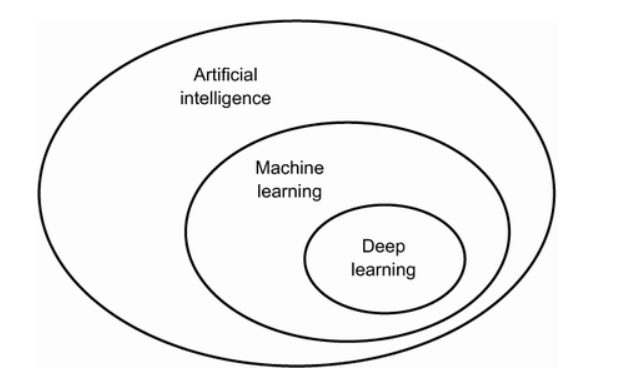
\includegraphics[scale=0.3]{ai-ml-dl.png}
    \caption{The AI, ML and DL Ecosystem}
    \label{fig:ai-ml-dl}
\end{figure}

Machine Learning (ML) and Deep Learning (DL) can be used interchangeably, however, there are differences, and it is worthwhile taking some time to look at them. 

\subsection{Machine Learning}
As seen, ML is a branch of AI and computer science which has a particular focus on using data-sets and various algorithms to mimic the way humans learn, and over time, improve the accuracy of the returned results. Machine leaning has really stated to come into its own as technological advances in areas such as data storage and processing power have increased. An example of this would be the Amazon recommendation engine. Amazon stores all the purchases, and all the searches it gets from all the users. When someone goes on to make a purchase, the Amazon recommendation engine will suggest items to that user, based on the purchases of other users who have bought similar items in the past.

Machine Learning will have an element of human input, more so than Deep Learning, as we will discuss later.

\section{Algorithms}
\subsubsection{Supervised Learning}
We will focus here in supervised learning, since labelled data will be used in the project. Specifically, we will focus on classification models, since we will be trying to classify if something is an obstacle or not.

Since we are aiming to classify if something is an obstacle or not, we are looking at two-class classification algorithms. Some of the algorithms we will investigate here are \cite{azure}:


\begin{itemize}
    \item Support Vector Machines
    \item Averaged Perceptron
    \item Decision Tree
    \item K-Nearest Neighbour
    \item Logistic Regression
    \item Boosted Decision Tree
    \item Neural Network
\end{itemize}


% \section*{Acknowledgment}


%\section*{References}
\printbibliography
\vspace{12pt}

\end{document}